%%%%%%%%%%%%
%
% Dashboard User Interface
%
%%%%%%%%%%%%

\chapter{Dashboard User Interface}
\label{ch:dashboard-ui}

This chapter introduces the visual structure of the CPI forecasting dashboard. The goal is to help the user understand where the controls are located, what each area of the interface does, and how the displayed output should be read during normal use.

\section{Layout Overview}

The dashboard uses a simple two-area structure:

\begin{itemize}
    \item \textbf{Sidebar (left):} model selection, confidence interval selection, and quick guidance text,
    \item \textbf{Main content area (right):} title, metrics, interactive chart, and interpretation panels.
\end{itemize}

This arrangement supports a natural user flow: choose settings on the left and interpret the resulting output on the right.

\section{Dashboard Layout Sketch}

Figure~\ref{fig:ui-sketch} provides a simplified structural sketch of the dashboard.

\begin{figure}[H]
    \centering
    \resizebox{0.96\textwidth}{!}{%
    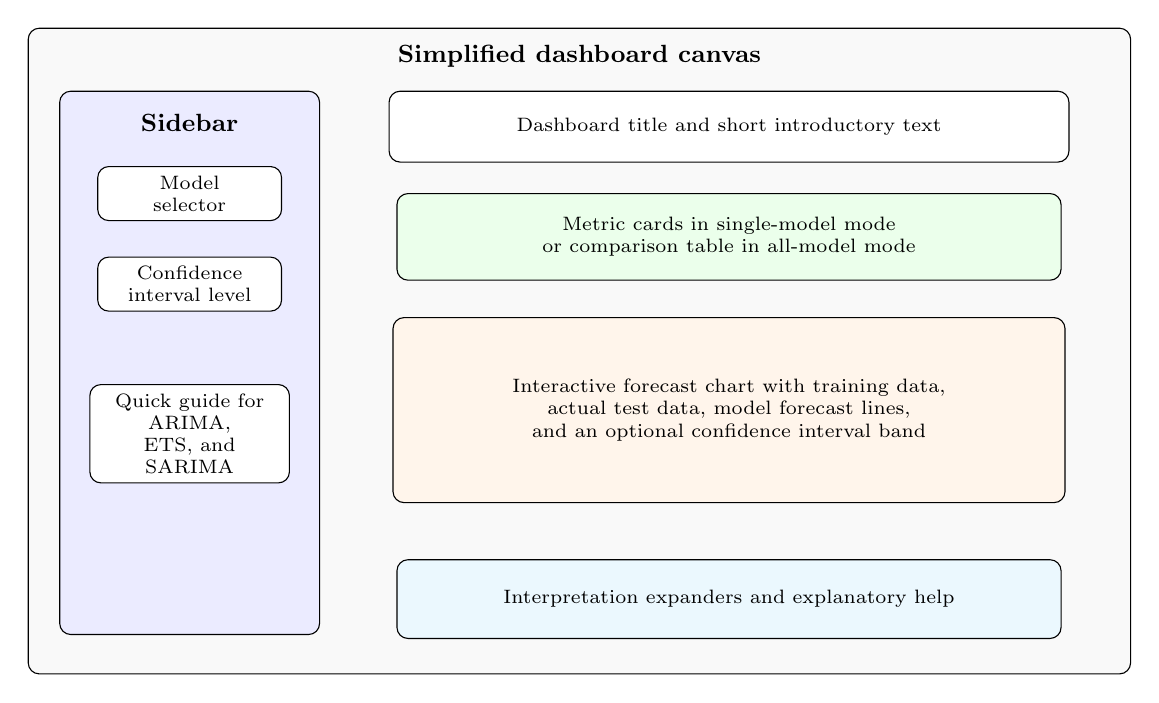
\begin{tikzpicture}[>=latex, every node/.style={font=\scriptsize}]
        \draw[rounded corners, fill=gray!5] (0,0) rectangle (14,8.2);
        \node[font=\small\bfseries] at (7,7.85) {Simplified dashboard canvas};

        \draw[fill=blue!8, rounded corners] (0.4,0.5) rectangle (3.7,7.4);
        \node[font=\small\bfseries] at (2.05,7.0) {Sidebar};
        \node[draw, fill=white, rounded corners, align=center, text width=2.1cm] at (2.05,6.1) {Model\\selector};
        \node[draw, fill=white, rounded corners, align=center, text width=2.1cm] at (2.05,4.95) {Confidence\\interval level};
        \node[draw, fill=white, rounded corners, align=center, text width=2.3cm] at (2.05,3.05) {Quick guide for\\ARIMA, ETS, and\\SARIMA};

        \node[draw, fill=white, rounded corners, align=center, text width=8.4cm, minimum height=0.9cm] at (8.9,6.95) {Dashboard title and short introductory text};
        \node[draw, fill=green!8, rounded corners, align=center, text width=8.2cm, minimum height=1.1cm] at (8.9,5.55) {Metric cards in single-model mode\\or comparison table in all-model mode};
        \node[draw, fill=orange!8, rounded corners, align=center, text width=8.3cm, minimum height=2.35cm] at (8.9,3.35) {Interactive forecast chart with training data,\\actual test data, model forecast lines,\\and an optional confidence interval band};
        \node[draw, fill=cyan!8, rounded corners, align=center, text width=8.2cm, minimum height=1.0cm] at (8.9,0.95) {Interpretation expanders and explanatory help};
    \end{tikzpicture}%
    }
    \caption{Simplified layout sketch of the Streamlit dashboard.}
    \label{fig:ui-sketch}
\end{figure}

\section{Dashboard Interface Screenshots}

Figures~\ref{fig:dashboard-full}, \ref{fig:dashboard-sidebar}, and \ref{fig:dashboard-main} document the running dashboard from the current repository state.

\begin{figure}[H]
    \centering
    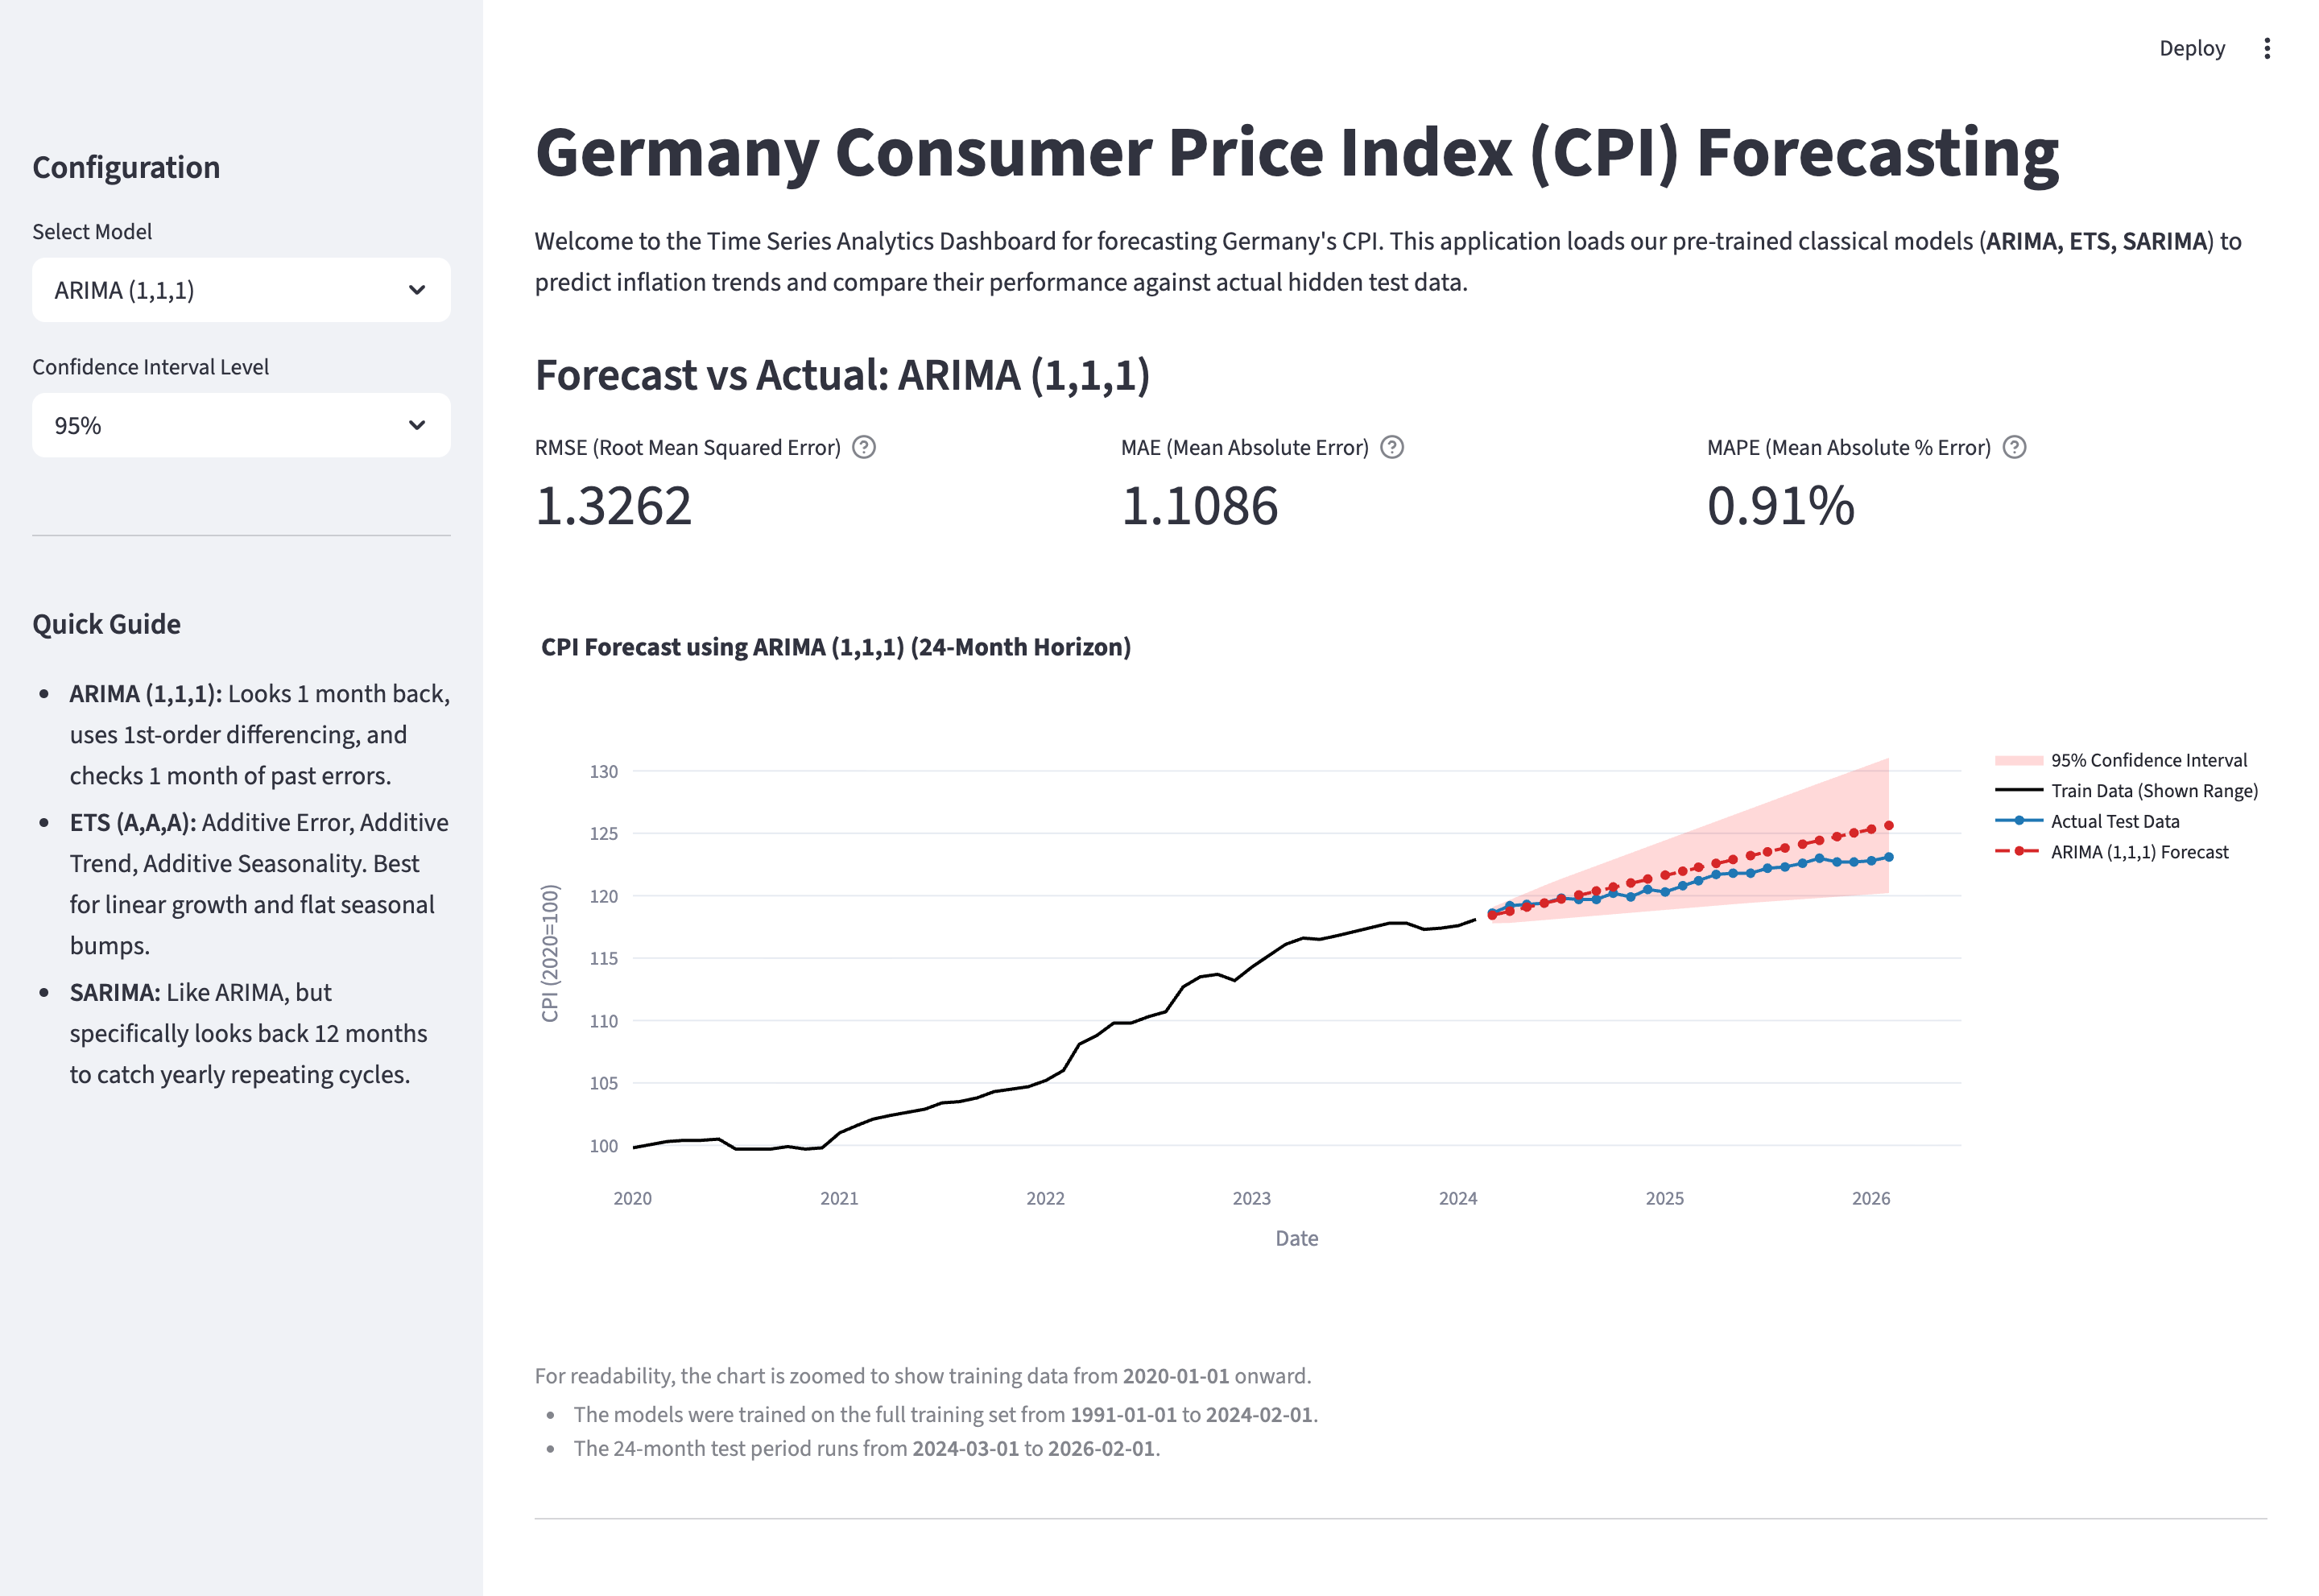
\includegraphics[width=0.98\textwidth]{Figures/dashboard-full.png}
    \caption{Full dashboard view in the browser.}
    \label{fig:dashboard-full}
\end{figure}

\begin{figure}[H]
    \centering
    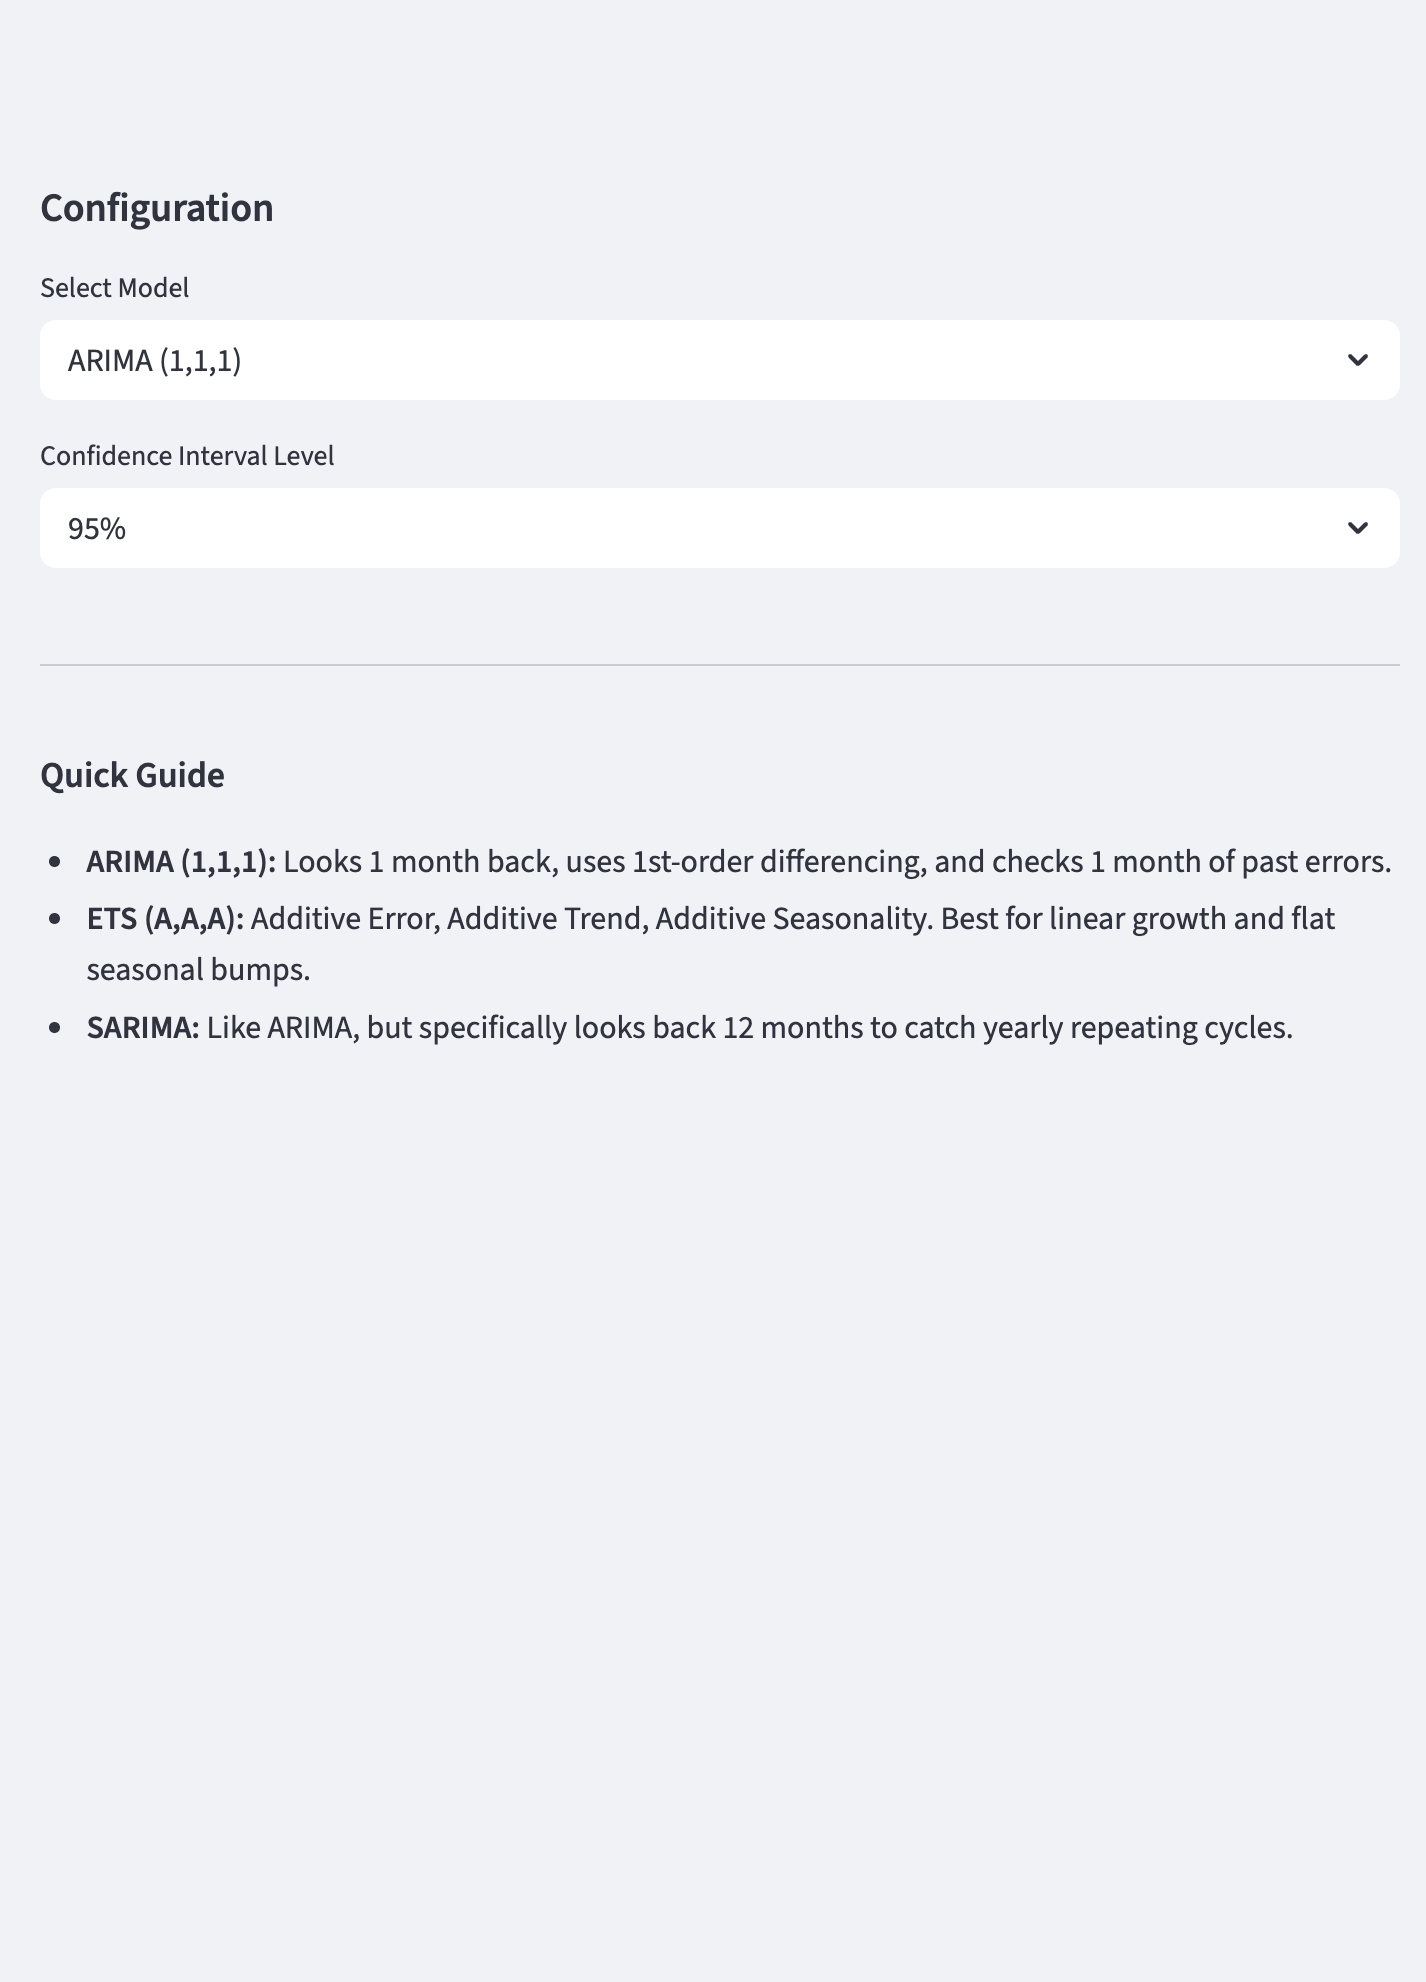
\includegraphics[width=0.5\textwidth]{Figures/dashboard-sidebar.png}
    \caption{Sidebar close-up with the model selector, confidence interval selector, and quick guide.}
    \label{fig:dashboard-sidebar}
\end{figure}

\begin{figure}[H]
    \centering
    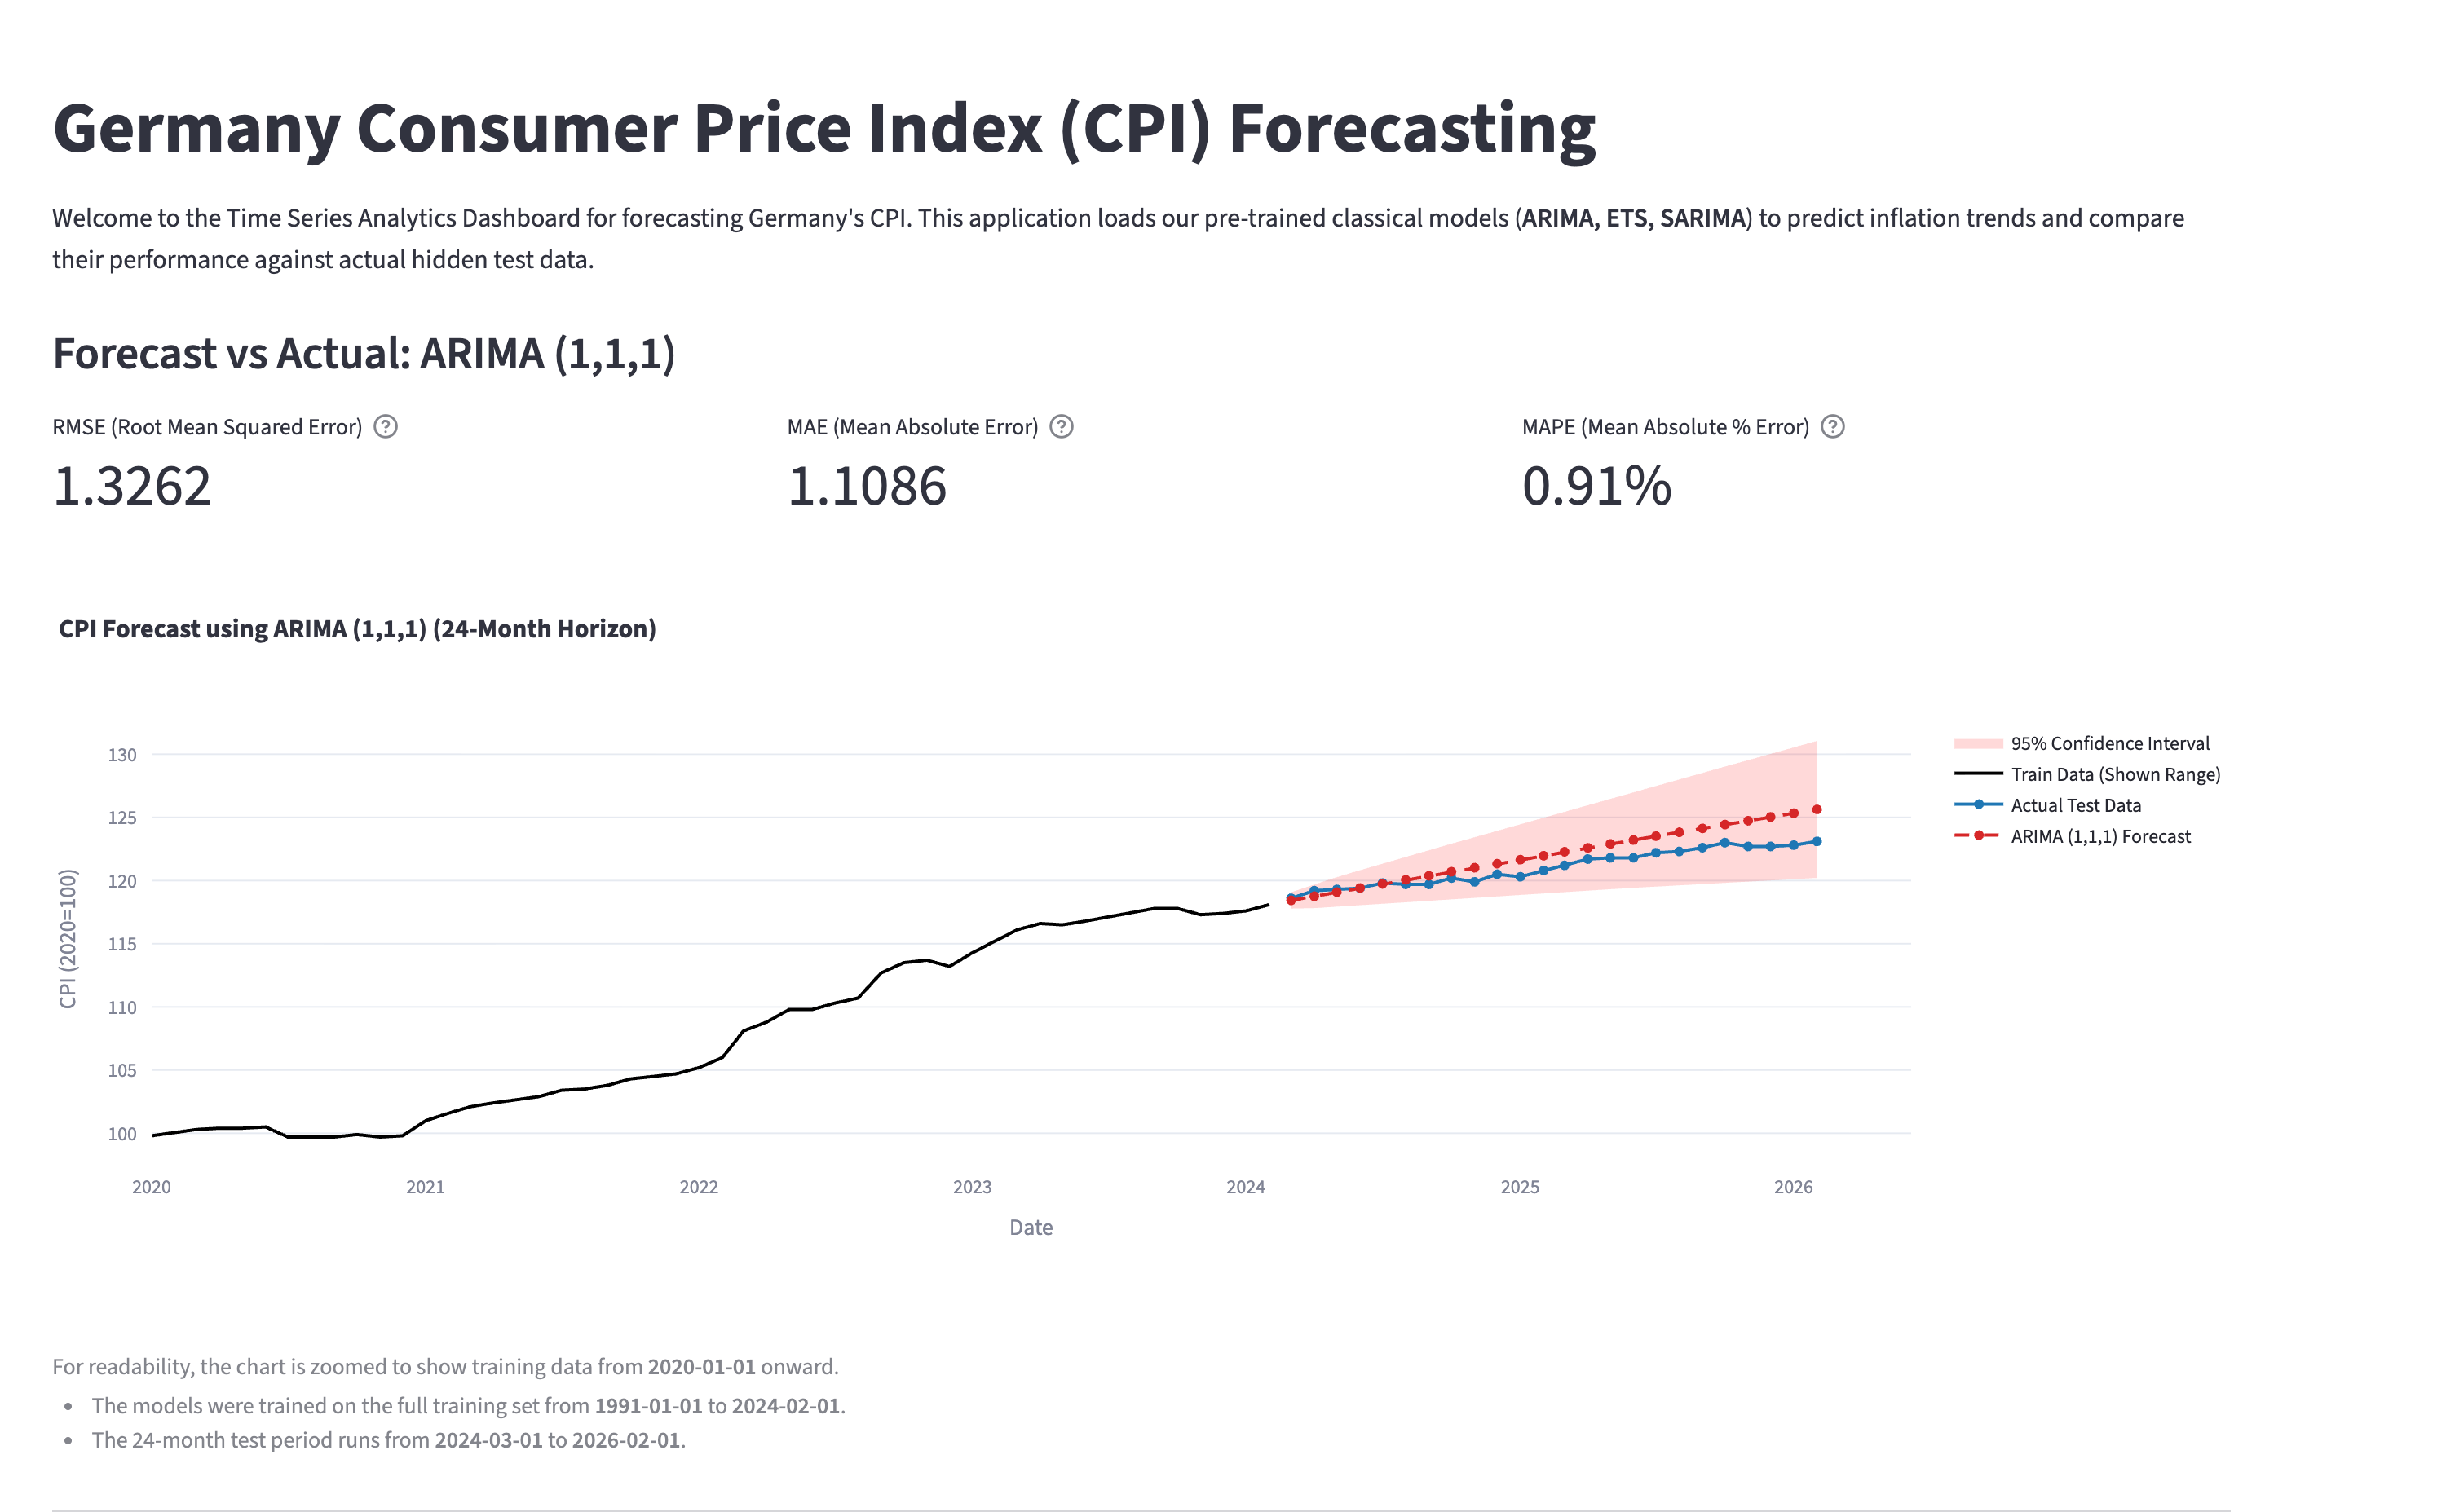
\includegraphics[width=0.98\textwidth]{Figures/dashboard-main.png}
    \caption{Main dashboard area with forecast metrics and the interactive chart.}
    \label{fig:dashboard-main}
\end{figure}

\section{Interface Walkthrough Table}

\begin{table}[H]
    \centering
    \renewcommand{\arraystretch}{1.25}
    \begin{tabularx}{\textwidth}{|L{3.3cm}|L{3.1cm}|X|}
        \hline
        \textbf{UI Element} & \textbf{Location} & \textbf{Purpose} \\
        \hline
        Select Model & Sidebar & Chooses between ARIMA, ETS, SARIMA, and comparison mode. \\
        \hline
        Confidence Interval Level & Sidebar & Changes the width of the uncertainty band in single-model mode. \\
        \hline
        Quick Guide & Sidebar & Gives a short plain-language explanation of each forecasting model. \\
        \hline
        Metric cards & Main area & Show RMSE, MAE, and MAPE for the selected model. \\
        \hline
        Comparison table & Main area & Replaces the metric cards when all-model comparison mode is selected. \\
        \hline
        Interactive chart & Main area & Displays training data, actual test data, forecasts, and confidence intervals. \\
        \hline
        Legend & Right side of chart & Allows traces to be hidden or shown interactively. \\
        \hline
        Plot toolbar & Upper chart area & Provides zoom, pan, reset, fullscreen, and plot download actions. \\
        \hline
        Interpretation expanders & Lower main area & Explain the forecasting pipeline, metrics, and confidence intervals in user-friendly language. \\
        \hline
    \end{tabularx}
    \caption{Dashboard interface elements and their user-facing purposes.}
    \label{tab:manual-ui-walkthrough}
\end{table}

\section{How to Read the Interface}

The normal sequence is simple:

\begin{enumerate}
    \item choose a model in the sidebar,
    \item choose a confidence interval level,
    \item read the metric area,
    \item inspect the forecast chart,
    \item open the explanation panels if more interpretation help is needed.
\end{enumerate}

When \texttt{Compare All Models} is selected, the metric cards are replaced by a comparison table and the chart overlays all model forecasts in one view. When one specific model is selected, the chart shows that model in detail together with its confidence interval band.

\begin{tcolorbox}[colback=purple!5!white, colframe=purple!75!black, title=Dashboard Reading Tips]
\begin{itemize}
    \item \textbf{Black line:} training data (recent history shown for clarity)
    \item \textbf{Blue line with markers:} actual test data (the "ground truth" hidden from models)
    \item \textbf{Red dashed line:} model forecast
    \item \textbf{Shaded band:} confidence interval (wider = more uncertainty)
\end{itemize}
\textbf{Tip:} If the red line closely follows the blue line, the model is performing well.
\end{tcolorbox}
